\documentclass{article}

\usepackage{Sweave}
\begin{document}
\Sconcordance{concordance:odds.tex:odds.Rnw:%
1 2 1 1 0 20 1 1 16 3 0 1 1 2 0 1 6 2 0 1 1 2 0 1 1 2 0 1 6 10 0 1 3 3 %
1 1 6 1 3 2 1}


\title{Odds of significance}

\author{Mc}
\maketitle
\section*{Introduction}
In simulations we checked the propability of an indicator (continuous or media-split) as the probability (frequency of runs) of being significant when it should be (latent effect size is greater than zero) over the probability of being significant when it should be not.
\section*{Setup}
\subsection*{Model}
Two continuous latent variables (\(\eta\) and \(\xi\) ) are created with N cases, sharing a correlation equal to \(\rho\). A measure \(x\) of \(\xi\) is created with reliability \(rel\), and then  is dichotomized accordingly to \(p\) \(1-p\) into \(c\). The correlations \( r_pe=r(\eta,x) \)  and \( r_pb=r(\eta,c) \) are computed, their p-value and significance (at .05) is recorded.
\subsection*{Design}
\(\rho=(0,.1,.2,.3,.4,.5,.6,.7) \)
\(rel=(0.3, 0.4 ,0.5, 0.6, 0.7 ,0.8 0.9) \) 

\subsection*{Propabilities as a functions of \(\rho\)}

The computation follows Jamie's computation at the last meeting. The probabilities are the following: \(f0\) is the number of times the indicator was the only one significant (so the other was not), \(f1\) is the probability of being the only one significant for a given \(\rho\). The probability \(P\) is \(P=f1+(f1+f0\))  


\begin{Schunk}
\begin{Soutput}
Number of times only Continuos was significant under the null hypothesis
\end{Soutput}
\begin{Soutput}
[1] 211
\end{Soutput}
\begin{Soutput}
Number of times only Categorical was significant under the null hypothesis
\end{Soutput}
\begin{Soutput}
[1] 217
\end{Soutput}
\begin{Soutput}
Odds of only Continuos  significant under true hypotheses
\end{Soutput}
\begin{Soutput}
  rho continuous categorical
1 0.1  0.6459732   0.5241228
2 0.2  0.7887888   0.5694444
3 0.3  0.8320064   0.5373134
4 0.4  0.8427720   0.4348958
5 0.5  0.8152364   0.4274406
6 0.6  0.7925270   0.3782235
7 0.7  0.7642458   0.3239875
\end{Soutput}
\end{Schunk}


\subsubsection*{Figure 1: Odds of being the only significant}

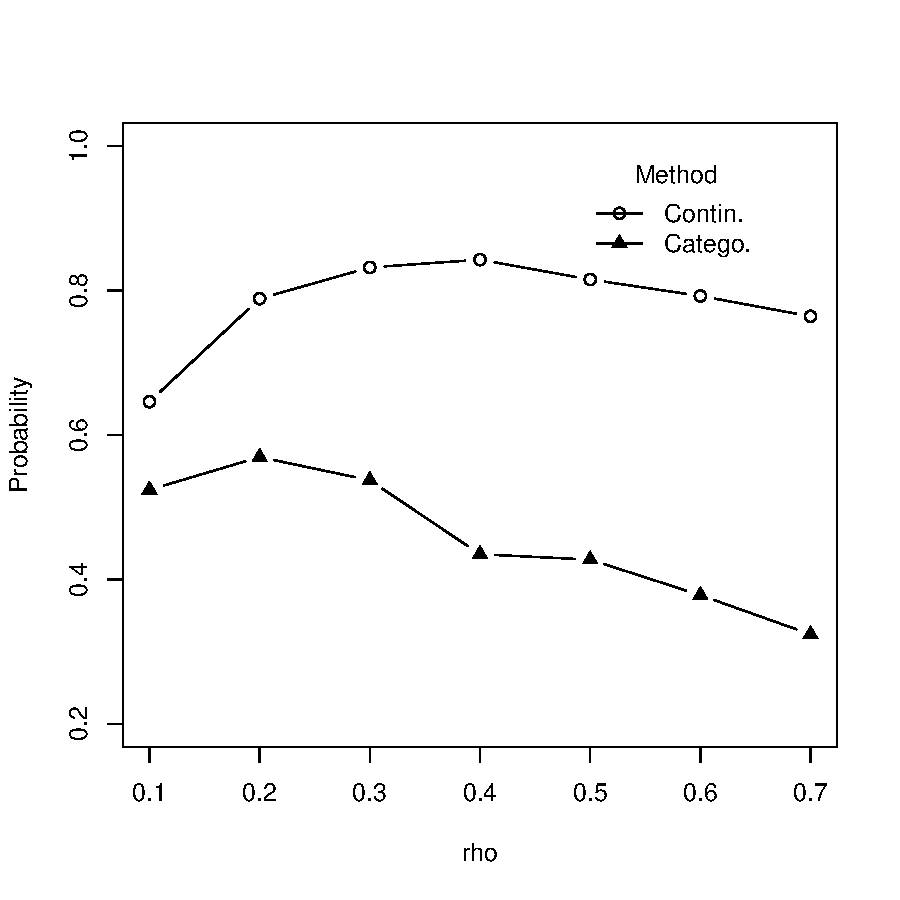
\includegraphics{odds-two}


\end{document}
